\documentclass[12pt,oneside,a4paper]{article}

\usepackage{custom}

\newcommand{\question}
{
\addtocounter{section}{1}
\section*{Question \thesection}
}

\newcommand{\myX}[2]{x_{#1,\text{#2}}}
\newcommand{\xSemaine}[1]{\myX{s}{#1}}
\newcommand{\xn}{\xSemaine{n}}
\newcommand{\xsup}{\xSemaine{sup}}
\newcommand{\xstock}{\xSemaine{stock}}
\newcommand{\xretard}{\xSemaine{retard}}
\newcommand{\xsst}{\xSemaine{sst}}
\newcommand{\xemb}{\xSemaine{emb}}
\newcommand{\xlic}{\xSemaine{lic}}

\newcommand{\texttts}[1]{{\small\texttt{#1}}}

\title{Projet d'optimisation}
\author{Groupe 1}
\date{\today}

\begin{document}

\maketitle

\question %1
\emph{Donnez une formulation linéaire (continue, sans variables entières) 
du problème de la planification de la ligne d'assemblage à personnel constant.
Décrivez successivement variables, contraintes et fonction objectif. 
A ce stade, le fait de ne pas imposer l'intégralité des variables 
vous parait-il problématique ?}

\subsection*{Variables}
Le tableau~\ref{tab:variablesQuestion1} contient les différentes variables $x_{s,\lambda}$
qui correspondent au nombre de smartphones pour chaque semaine $s$
avec la caractéristique $\lambda$.

\begin{table}[h]
  \begin{center}
  \begin{tabular}{|c|l|}
    \hline
    Variable & Caractéristiques des smartphones \\
    \hline
    \hline
    $\xn$ & Produits au \emph{salaire normal}. \\
    \hline
    $\xsup$ & Produits pendant les \emph{heures supplémentaires}. \\
    \hline
    $\xstock$ & Conservés en \emph{stock}. \\
    \hline
    $\xretard$ & Vendus une semaine en \emph{retard}. \\
    \hline
    $\xsst$ & Sous-traités. \\
    \hline
  \end{tabular}
  \caption{Variables de la modélisation de la ligne d'assemblage simple.}
  \label{tab:variablesQuestion1}
  \end{center}
\end{table}

\subsection*{Contraintes}
Voici les contraintes du problème de la planification 
de la ligne d’assemblage à personnel constant.
On pose que $\Delta x_{s,\lambda} = x_{s,\lambda} - x_{s-1,\lambda}$.
\begin{align*}
  \Delta\xstock + \texttts{demande}(s) &= \xn + \xsup 
  + \xretard + \xsst - \myX{s-1}{retard} &\forall s \\
  \myX{0}{n}&= 0 \\
  \myX{0}{sup}&= 0 \\
  \myX{0}{stock} &= \texttts{stock-initial} \\
  \myX{0}{retard}&= 0 \\
  \myX{0}{sst}&= 0 \\
  \myX{T}{stock} &= \texttts{stock-initial} \\
  \myX{T}{retard}&= 0 \\
  \myX{s-1}{retard} + \Delta\xstock &\leq \xn + \xsup + \xsst &\forall s \\
  \xn &\leq 35\cdot \texttts{nb\_ouvriers}/ d_{a,h}
  &\forall s \\
  \xsup &\leq \texttts{nb\_max\_heure\_sup}\cdot\texttts{nb\_ouvriers}/ d_{a,h}
  &\forall s \\
  \xsst &\leq \texttts{nb\_max\_sous\_traitant} &\forall s \\
  x_s &\geq 0 &\forall s
\end{align*}

\subsection*{Fonction objectif}
\[
  \mbox{minimiser } 
  \sum_{s=1}^{T} 
  c_m\, \xn + (c_m + d_{a,h} \, c_{hs})\, \xsup
  + c_s\, \xstock + c_r\, \xretard + c_{sst}\, \xsst
\]
Le tableau~\ref{tab:constantesQuestion1} contient les abréviations
des constantes utilisées.
\begin{table}[h]
  \begin{center}
  \begin{tabular}{|c|l|}
    \hline
    Paramètre & Constante représentée \\
    \hline
    \hline
    $c_m$ & \texttt{cout\_materiaux} \\
    \hline
    $c_{hs}$ & \texttt{cout\_heure\_sup} \\
    \hline
    $c_s$ & \texttt{cout\_stockage} \\
    \hline
    $c_r$ & \texttt{cout\_retard} \\
    \hline
    $c_{sst}$ & \texttt{cout\_sous\_traitant} \\
    \hline
    $d_{a,h}$ & \texttt{duree\_assemblage}/60 \\
    \hline
  \end{tabular}
  \caption{Constantes de la modélisation de la ligne d'assemblage simple.}
  \label{tab:constantesQuestion1}
  \end{center}
\end{table}

A ce stade, le fait de ne pas imposer l'intégralité des variables
parait problèmatique dans le sens où les solutions ne sont pas 
garanties d'être entières. Ce qui n'est pas envisageable 
vu que celles-ci représentent des quantités de smartphones.
Par exemple, 
$\xn$ ne sera probablement pas entier si $1/d_{a,h}$ ne l'est pas.
% TODO autre mot que problablement ? "il est possible que" 

\question %2
\emph{Démontrez que, sous certaines hypothèses raisonnables, 
il est possible de garantir que votre modèle linéaire continu admette toujours
une solution entière, c'est-à-dire ne comportant que des quantités produites
entières chaque semaine. 
L'une de ces hypothèses est l'intégralité de la demande chaque semaine ; 
quelles sont les autres ?}

Il est possible de garantir que notre modèle linéaire continu
admette toujours une solution entière sous certaines hypothèses.
Une première hypothèse est que tous les éléments du 
vecteur \texttt{demande} soient entiers.
Il faut également que les constantes \texttt{stock-initial},
\texttt{nb\_max\_heure\_sup}, \texttt{nb\_max\_sous\_traitant},
\texttt{nb\_ouvriers} et $1/d_{a,h}$ soient entières.
% TODO nécéssaire de spécifier même celles qui parraissent évidente? 

\subsubsection*{Preuve}
Pour le prouver, nous allons reformuler notre problème sous la forme d'un problème de flot de coût minimum.
Soit le graphe orienté $G(V,E)$, 
où $V$ représente l'ensemble des noeuds et $E$ l'ensemble des arrêtes.
Il est utile à ce stade de s'aider d'un schéma représentant le graphe. 
Celui-ci est repris à la figure~\ref{fig:schemaFlot}.
$V$ compte un noeud pour chaque semaine et un noeud initial.
On a donc $V := {0, 1, 2, ..., T}$
où $0$ est le noeud initial et $s$ est le noeud de la semaine $s$.
Définissons maintenant les arrêtes de notre graphe.
Pour le noeud $0$, on définit 
\[ V^{-}(0) = \{s_1, s_2, s_3 \, \forall s \ne 0\} \]
avec
\[ \{(0, s_1), (0, s_2), (0, s_3)\} \in E \, \forall s. \]
$s_1$, $s_2$, $s_3$ représentent les différentes manières de produire les smartphones, c'est-à-dire les ouvriers au salaire normal, les ouvriers au salaire des heures supplémentaires et la sous-traitance.
Il y a donc trois arcs entre les noeuds $0$ et $s$.
Pour le noeud initial,
\[ V^{+}(0) = \emptyset \]
Définissons ensuite les arrêtes des noeuds corrspondnats aux semaines
\[ V^{-}(s) = \{s+1\} \qquad \forall s \ne 0 \]
avec 
\[ \{(s, s+1)\} \in E \qquad \forall s \ne 0, T \]
Et,
\[ V^{+}(s) = \{s-1\} \qquad \forall s \ne 0 \]
avec
\[ \{(s, s-1)\} \in E \qquad \forall s \ne 0, 1 \]
Nous devons encore définir les termes sources pour chaques noeuds ainsi que les capacités maximales pour chaque arc.
Soit
\[ b_s = - \texttts{demande}(s) \qquad s \in V \backslash \{0\} \]
Et 
\[ b_0 = \sum_{s=1}^{T} \texttts{demande}(s) \]  
On a aussi
\[ b_1 = \texttts{stock\_initial} \]
Et
\[ b_T = - \texttts{stock\_initial} \]
Soient $h_{ij}$ avec $(i, j) \in E$ les capacités maximales dans l'arc $(i, j)$.
On a $\, \forall s \ne 0$ 
\begin{align*}
  h_{0, s_1} &= 35\cdot \texttts{nb\_ouvriers}/ d_{a,h} \\
  h_{0, s_2} &= \texttts{nb\_max\_heure\_sup}\cdot\texttts{nb\_ouvriers}/ d_{a,h} \\
  h_{0, s_3} &= \texttts{nb\_max\_sous\_traitant} 
\end{align*}
Le graphe maintenant défini, 
on peut définir le problème de minimisation suivant :
\paragraph{Variables}
Soit $x_{ij}$ le flot dans l'arc $(i, j)$.
\paragraph{Objectif}
Le coût total est minimisé.
\[ \sum_{(i, j) \in E} c_{ij} x_{ij} \]
\paragraph{Equations} Le flot est conservé en chaque noeud
\[ \sum_{k \in V^{+}(i)} x_{ik} - \sum_{k \in V^{-}(i)} x_{ki} 
  = b_i \qquad i \in V
\]
Les capacités maximales ne sont pas dépassées
\[ 0 \leq x_{ij} \leq h_{ij} \qquad (i, j) \in E \]

On peut maintenant utiliser le théorème suivant pour conclure que, si nos hypothèses sont vérifiées, notre problème admettra au moins une solution entière.
\paragraph{Théorème}
Si les demandes $b_i$ et les capcités $h_{ij}$ d'un problème de flot de coût minimum sont entières alors il existe une solution optimale entière.

\begin{figure}[H]
	\centering
		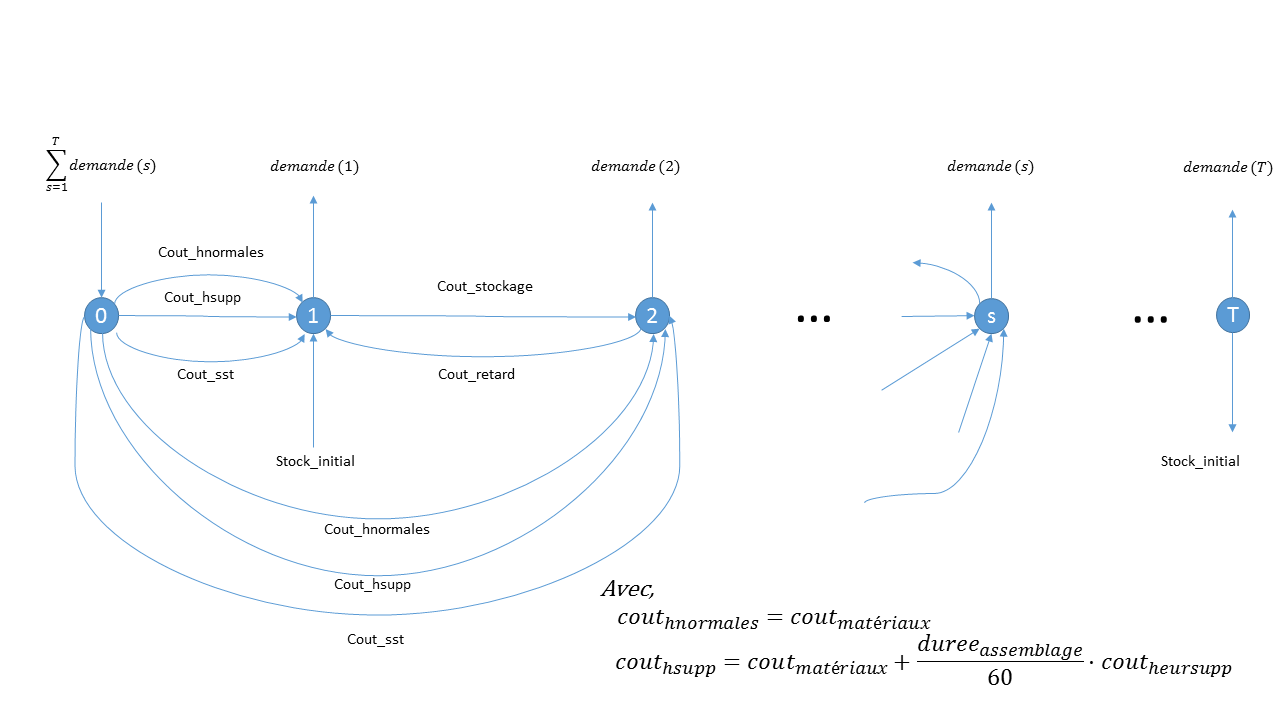
\includegraphics[scale = 0.5]{Schema_flot.png}
	\caption{Schéma représentant le graphe utilisé pour définir 
  le problème de flot de coût minimal.}
	\label{fig:schemaFlot}
\end{figure}

\question %3
\emph{Implémentez sous MATLAB ce modèle linéaire continu, 
et calculez la solution correspondant aux données fournies sur icampus 
(utilisez la fonction \texttt{linprog}). 
Commentez l'allure de la solution obtenue.}

Notre implémentation se trouve dans le fichier \texttt{question3.m}.
Il nous parait important d'expliquer en quelques mots le r\^ole
de la fonction \texttt{kron}.
Celle-ci effectue le produit tensoriel de Kronecker entre deux matrices.
C'est-à-dire que pour \texttt{kron(A,B)},
chaque élément de $A$ multiplie la matrice $B$.
En l'utilisant de manière appropriée avec des matrices nulles et diagonales,
on peut effectuer un remplissage des matrices des contraintes très efficace. 

Les résultats obtenus sont représentés graphiquement 
à la figure~\ref{fig:grapheProduction}. 
Comme on pouvait s'y attendre, la solution optimale utilise presque chaque
semaine au maximum la ressource la moins chère,
en l'occurence la production par les ouvriers payés au salaire normal.
On observe également que la solution optimale constitue un stock dans la première partie de la planification pour faire face au pic de demande 
situé entre les semaines 5 et 8.
La demande est particulièrement importante à la semaine 7,
et on voit que notre stock constitué s'épuise totalement lors de cette semaine.
On commence également à avoir recours au retard.

\begin{figure}[H]
  \begin{center}
    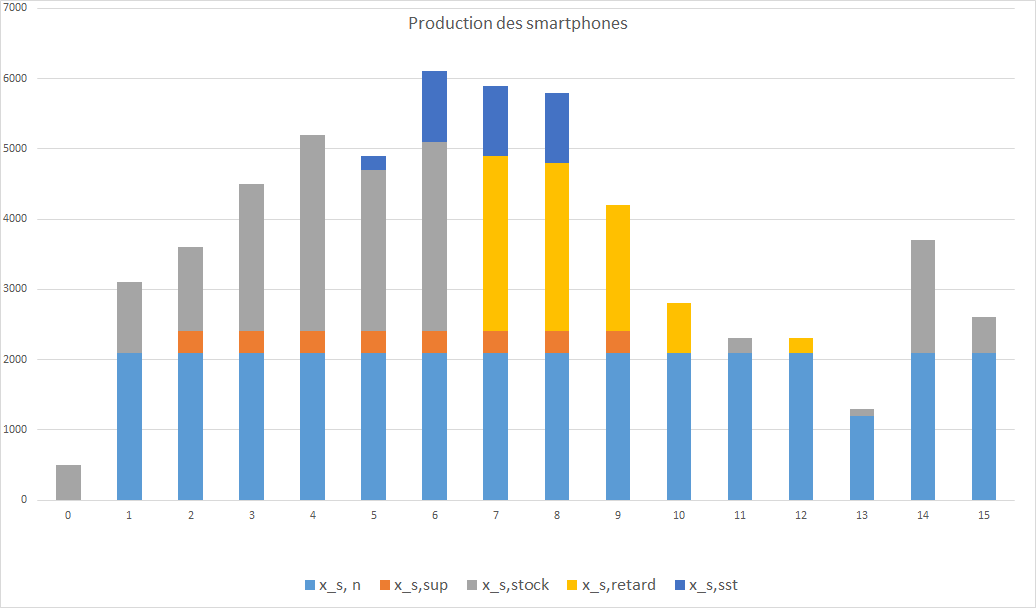
\includegraphics[scale = 0.8]{grapheProduction.png}
	  \caption{Répartition du moyen de production des smartphones en fonction des semaines.}
	  \label{fig:grapheProduction}
  \end{center}
\end{figure}

\question %4
\emph{Décrivez une procédure permettant, avec le moins de nouveaux calculs
possibles, d'évaluer les conséquences sur la fonction objectif d’une petite
variation de la demande prévue. Plus précisément, analysez l'effet du
remplacement du vecteur \texttt{demande} 
par le vecteur \texttt{demande + epsilon * delta\textunderscore demande} 
où \texttt{delta\textunderscore demande} est un vecteur de perturbation 
sur la demande, 
et \texttt{epsilon} est un paramètre scalaire dont la valeur est faible.}

Le dual du problème nous permet d'évaluer assez simplement
les conséquences sur la fonction objectif
d'une petite variation de la demande prévue.

En effet, notre problème peut être simplifié sous la forme
\begin{align*} 
	\text{minimiser } c^T x \\
	a_i^T x &= b_i  & i = 1,...,T,...,T+3 \\
  a_i^T x &\leq b_i & i = T+4,...,end \\
	x_j &\geq 0 & \forall j
\end{align*}
On obtient ensuite sa forme duale
\begin{align*} 
	\text{maximiser } b^T y \\
	y_i &\text{ libre} & i = 1,...,T,...,T+3 \\
  y_i &\leq 0 & i = T+4,...,end \\
  A_j^T y &\leq c_j & \forall j
\end{align*}

%Une partie du vecteur $b$ (et plus précisement les $T$ premiers éléments)
%correspond à la demande.
On remarque qu'une perturbation des contraintes dans le problème primal
correspond à une perturbation de la fonction objectif dans le problème dual.
Il nous suffit donc simplement de calculer une solution optimale du dual $y^{*}$
puis d'effectuer le produit scalaire
\[ \Delta z^{*} = (\Delta b)^T y^{*} \]
pour chaque perturbation $\Delta b$ pour conna\^itre l'impact $\Delta z^{*}$
sur le cout.

\question %5
\emph{Testez sous MATLAB la procédure du point précédent avec les données
fournies. Comparez ensuite la prédiction obtenue par cette procédure
avec la valeur obtenue en résolvant à nouveau complètement le modèle,
et ce pour un échantillon de valeurs du paramètre \texttt{epsilon} comprises
entre $0$ et $1$ (par exemple \texttt{0:.1:1}). 
Commentez (éventuellement en vous aidant d'un graphique).}

Comparaison À FAIRE.

Notre fonction \texttt{compareDuality.m} permet de prouver l'efficacité
du problème dual lorsqu'on perturbe le vecteur des contraintes.
En effet, si l'on décide d'analyser via le problème primal ce qu'il 
se passe lorsque les contraintes sont modifiées, il est nécessaire de 
résoudre le problème à chaque perturbation 
(plusieurs appels à \texttt{linprog}).
Tandis que pour le problème dual,
il suffit d'effectuer plusieurs combinaisons linéaires de la fonction objectif
avec \emph{une seule} solution $y^{*}$ 
(c'est-à-dire un apppel à \texttt{linprog}).
On retrouve les résultats des tests d'efficacité
sur le graphe de la figure~\ref{fig:efficiencyDual}.

\begin{figure}
  \begin{center}
    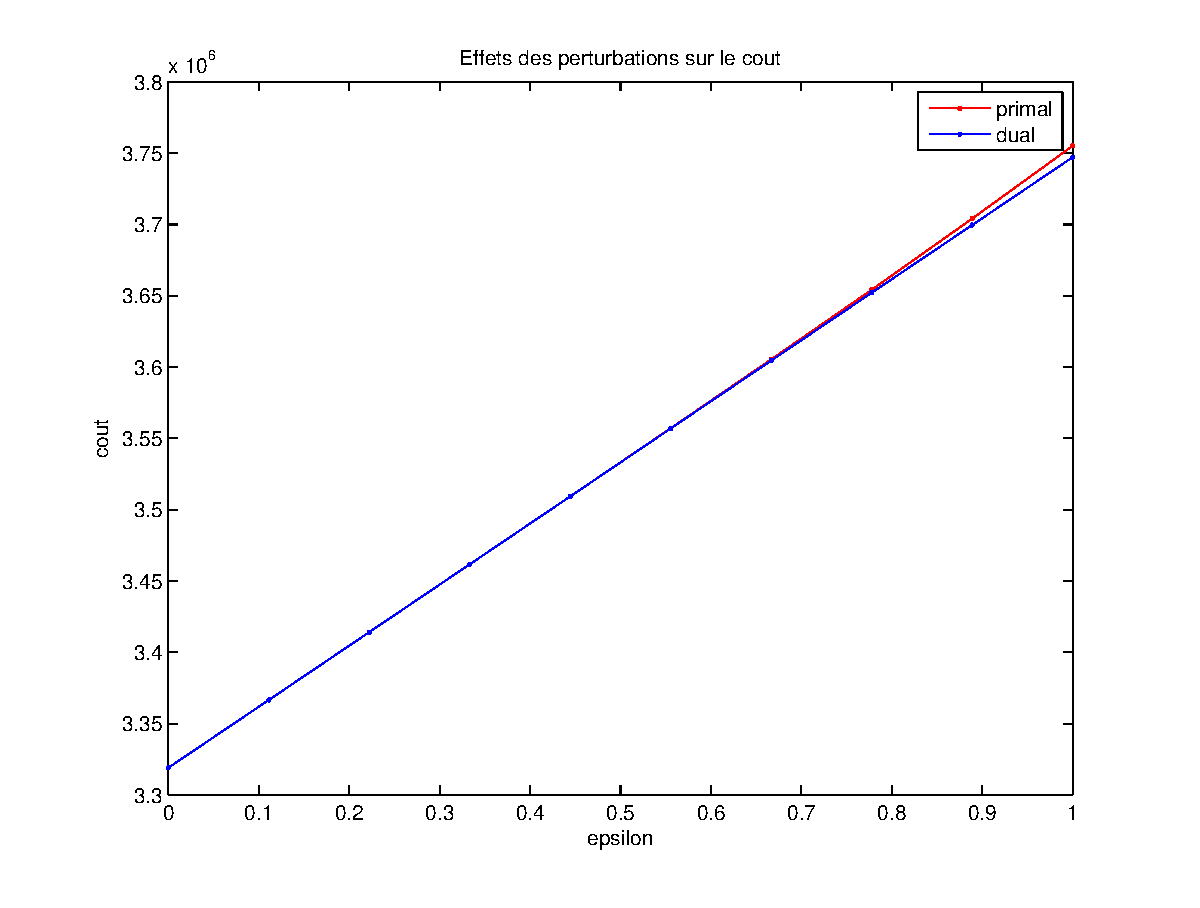
\includegraphics[scale=0.6]{img/responseToPerturbations.eps}
    \caption{Comparaison de la réponse aux perturbations du primal 
    et dual. On remarque que les valeurs restent égales jusqu'à 
    $\epsilon \approx 0.6$.}
    \label{fig:responseToPerturbations}
  \end{center}
\end{figure}

\begin{figure}
  \begin{center}
    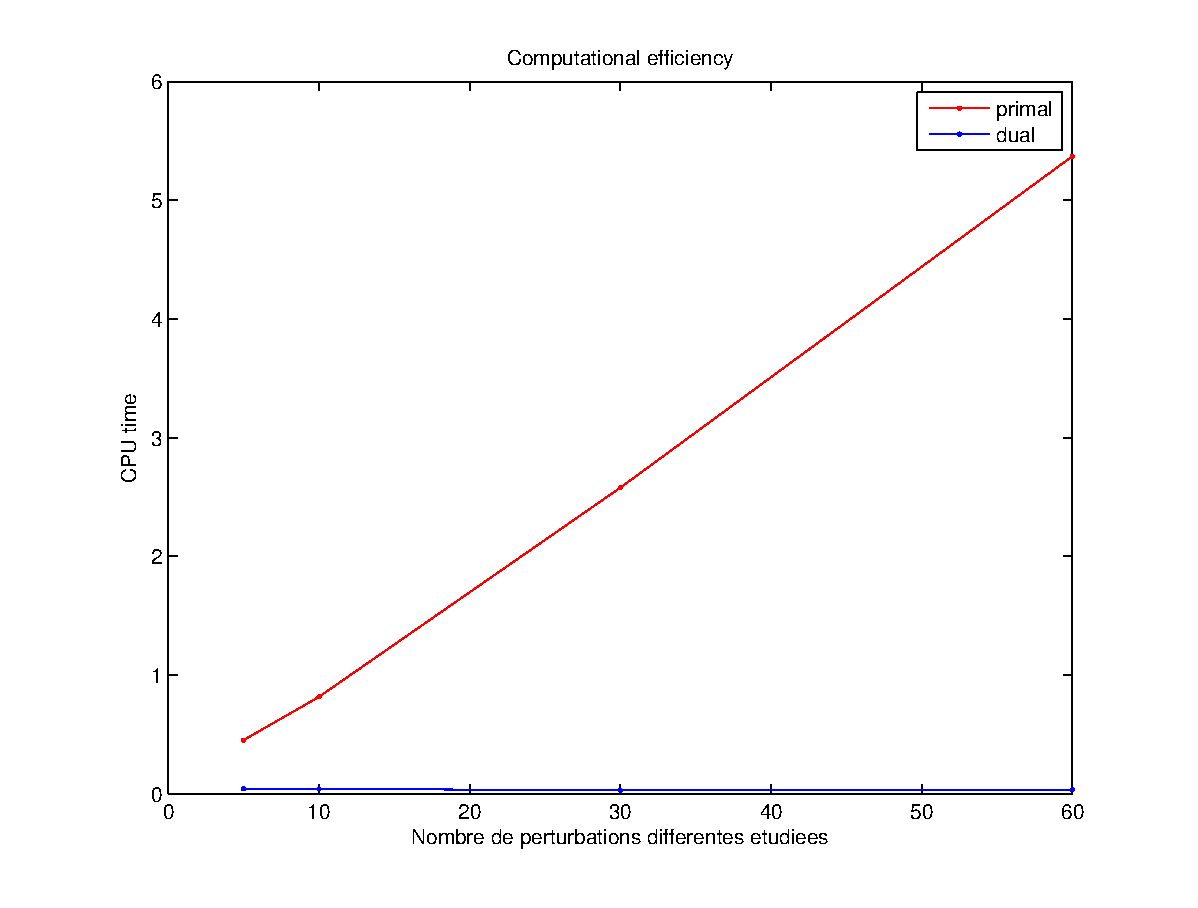
\includegraphics[scale=0.6]{img/efficiencyDual.eps}
    \caption{Comparaison de l'efficacité du primal et dual lors de
    l'analyse de perturbations sur les contraintes.}
    \label{fig:efficiencyDual}
  \end{center}
\end{figure}

\question %6
\emph{Décrivez (sans l'implémenter) l'adaptation qu'il serait nécessaire à
apporter au modèle si le coût de l'heure supplémentaire pris en compte était
variable. Plus concrètement, considérez qu'après la première heure
supplémentaire (facturée au coût horaire \texttt{cout\textunderscore
heure\textunderscore sup} standard), chaque heure supplémentaire
(éventuellement) est facturée à un coût horaire supérieur de $5 \%$ 
à celui de l'heure supplémentaire précédente. 
Est-il toujours possible de formuler (ou reformuler) 
le problème sous forme linéaire ? Expliquez. 
Et que se passerait-il si le coût horaire des supplémentaires \emph{diminuait}
lorsque le nombre d'heure prestées augmente ? Justifiez.}

Si le coût des heures supplémentaires n'est plus constant mais augmente au fur et à mesure de leur utilisation, 
le coût de celles-ci dépenderait directement du nombre de smartphones 
produits de cette manière.

En effet, on peut réécrire notre fonction objectif comme
\[
  \mbox{minimiser } 
  \sum_{s=1}^{T} 
  c_m\, \xn + c_m \, \xsup + \mathcal{C}_{hs} (\xsup)
  + c_s\, \xstock + c_r\, \xretard + c_{sst}\, \xsst
\]
avec
\[
  \mathcal{C}_{hs} (\xsup) = \texttts{cout\_heure\_sup} \cdot
  \sum_{i=0}^{\alpha} \binom{\alpha}{i} (0.05)^{i} 
\]
Par soucis de lisibilité, on a posé
\[ \alpha = \xsup \, d_{a,h} - 1 \]
$\alpha$ correspond donc au nombre d'heures supplémentaires qui auront
un cout différent de \texttt{cout\_heure\_sup}.

On remarque immédiatement que la fonction $\mathcal{C}_{hs}$
est \emph{non-linéaire} en $\xsup$ puisque 
\[ \binom{\alpha}{i} =\frac{\alpha !}{i!\,(\alpha-i)!} \]

Si le coût des heures supplémentaires \emph{augmentent} avec un taux de $0.05$,
la fonction objectif devient 

avec

Ce modèle n'est plus linéaire.

De même, si le coût des heures supplémentaires \emph{diminuait} 
avec un taux de $0.05$,
on aurait
\[
  c_{hs} (\xsup) = \texttts{cout\_heure\_sup} \cdot
  \sum_{i=0}^{\alpha} (-1)^i(0.05)^{i} \,   \binom{\alpha}{i}
\]


\question %7
\emph{Donnez à présent une formulation linéaire (continue, sans variables
entières) du problème de la planification de la ligne d'assemblage
incluant le gestion du personnel, en vous basant sur le modèle déjà 
construit à la Question 1. Décrivez successivement variables, 
contraintes et fonction objectif.}

Le nombre d'ouvriers n'étant plus constant, nous allons rajouter deux variables
par semaine pour modéliser le problème :
\begin{itemize}
  \item[$\diamond$] $\xemb$ le nombre d'ouvriers embauchés au début de la semaine $s$
  \item[$\diamond$] $\xlic$ le nombre d'ouvriers licienciés au début de la semaine $s$.
\end{itemize}
Dans la fonction objectif, il faut maintenant tenir compte du cout de 
ces recrutements et ces licenciements 
ainsi que du coût du salaire des ouvriers, non constant.

En ce qui concerne les contraintes, il faut modifier celles sur 
le nombre de smartphones maximum produits dans l'entreprise. 
Il faut également ajouter les contraintes correspondants 
au nombre d'ouvriers (maximum et minimum).

\subsection*{Fonction objectif}
\begin{align*}
  \mbox{minimiser } 
  \sum_{s=1}^{T} 
  c_m\, \xn + (c_m + d_{a,h} \, c_{hs})\, \xsup
  + c_s\, \xstock + c_r\, \xretard + c_{sst}\, \xsst \\
  + 35 \, c_{h} \, (n_{ouv} + \sum_{i=1}^{s} x_{i,emb} - x_{i,lic}) 
  + c_{emb} \, \xemb + c_{lic} \, x_{i,lic}
\end{align*}

Le tableau~\ref{tab:constantesQuestion7} contient les nouvelles abréviations
des constantes utilisées.
\begin{table}[h]
  \begin{center}
  \begin{tabular}{|c|l|}
    \hline
    Paramètre & Constante représentée \\
    \hline
    \hline
    $c_{h}$ & \texttt{cout\_horaire} \\
    \hline
    $c_{emb}$ & \texttt{cout\_embauche} \\
    \hline
    $c_{lic}$ & \texttt{cout\_licenciement} \\
    \hline
    $n_{ouv}$ & \texttt{nb\_ouvriers} \\
    \hline
  \end{tabular}
  \caption{Constantes de la modélisation de la ligne d'assemblage
  avec gestion du personnel.}
  \label{tab:constantesQuestion7}
  \end{center}
\end{table}

\subsection*{Contraintes}
Voici les contraintes du problème de la planification 
de la ligne d’assemblage à personnel variable.
\begin{align*}
  \Delta\xstock + \texttts{demande}(s) &= \xn + \xsup 
  + \xretard + \xsst - \myX{s-1}{retard} &\forall s \\
  \myX{0}{n}&= 0 \\
  \myX{0}{sup}&= 0 \\
  \myX{0}{stock} &= \texttts{stock-initial} \\
  \myX{0}{retard}&= 0 \\
  \myX{0}{sst}&= 0 \\
  \myX{T}{stock} &= \texttts{stock-initial} \\
  \myX{T}{retard}&= 0 \\
  \myX{s-1}{retard} + \Delta\xstock &\leq \xn + \xsup + \xsst &\forall s \\
  \xn &\leq 35\cdot (n_{ouv} + \sum_{i=1}^{s} x_{i,emb} - x_{i,lic})/ d_{a,h}
  &\forall s \\
  \xsup &\leq \texttts{nb\_max\_heure\_sup}\cdot \left(n_{ouv} + \sum_{i=1}^{s} x_{i,emb} - x_{i,lic} \right)/ d_{a,h}
  &\forall s \\
  \xsst &\leq \texttts{nb\_max\_sous\_traitant} &\forall s \\
  n_{ouv} + \sum_{i=1}^{s} x_{i,emb} - x_{i,lic} &\leq \texttts{nb\_max\_ouvriers}  &\forall s \\
  x_s &\geq 0 &\forall s
\end{align*}

\end{document}